\section{Widoki aplikacji i opis ich działania}

\subsection{Widok główny}
Widok główny pozwala na ogólną prezentację danych z czujników z domyślnego zakresu 24-godzin z zaznaczeniem, w której sali znajduje się dany czujnik. 
Użytkownik posiada opcję wyboru jaki typ odczytu będzie prezentowany na wykresie (temperatura, wilgotność względna, stężenie CO2), zarówno indywidualnie 
poprzez interakcję z guzikami "radiowymi" dla każdego czujnika/sali oraz dla każdego z czujników jednocześnie poprzez wybranie typu
w liście rozwijanej. 

\begin{figure}[H]
    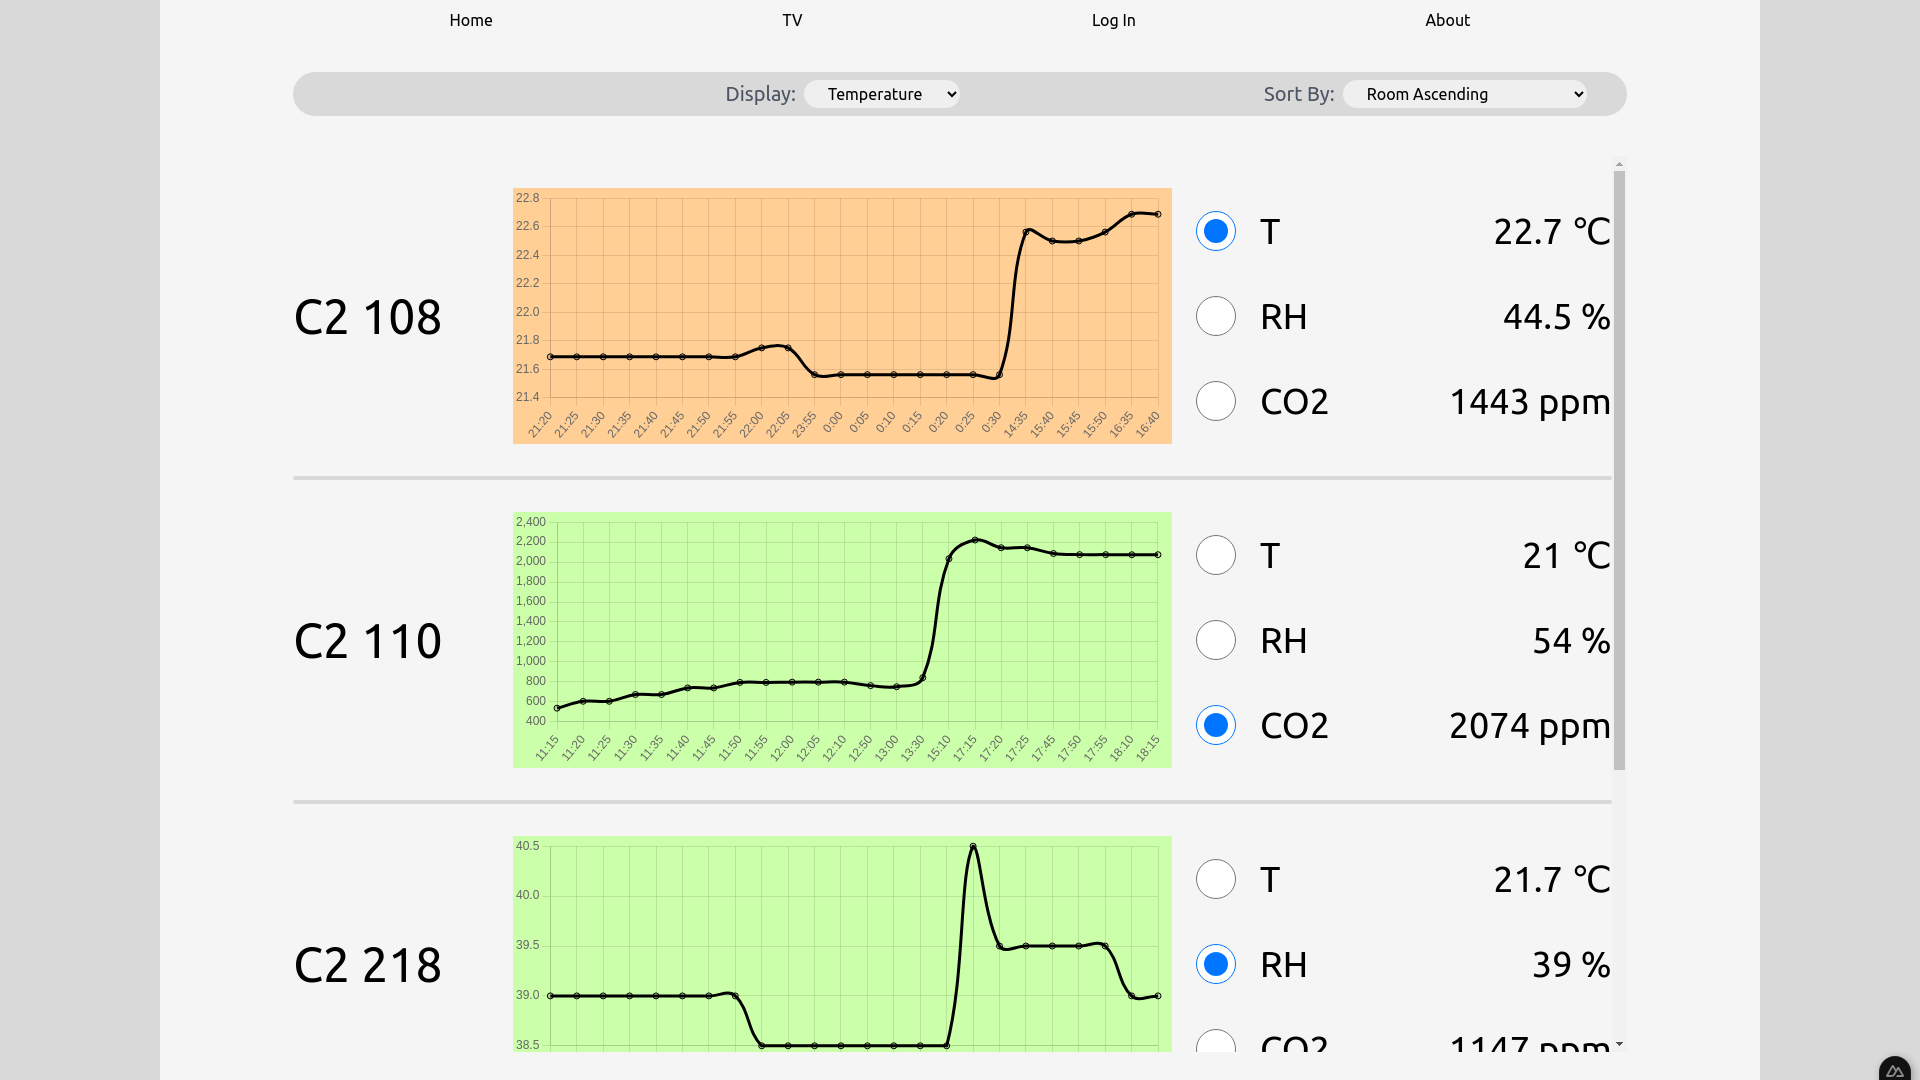
\includegraphics[width=\textwidth]{zdj/app/main.png}
    \caption{Zrzut ekranu przedstawiający widok główny}
\end{figure}

Dane z czujników przedstawione na wykresach są aktualizowane tak często, jak stają się one dostępne, biorąc pod uwagę opóźnienia związane
z cyklicznym odpytywaniem serwera o nowe dane czy straty czasu związane z samym przesyłem danych. Stan jakości powietrza jest dodatkowo
odzwierciedlany poprzez zmienne tło na wykresach - zielony oznacza optymalną wartość parametru, pomarańczowy stan bliski wartościom powodującym
dyskomfort bądź negatywnie wpływającym na zdrowie, zaś czerwony wartości niezalecane przy długotrwałym przebywaniu w pomieszczeniu.

Przedziały zostały dobrane na podstawie rozdziału "\nameref{opis-parametrow}"

\subsection{Widok szczegółów}

Po kliknięciu na dowolny z elementów odpowiadających czujnikowi na poprzednim widoku ukazuje się nam widok szczegółów danego czujnika. Można tutaj odczytać
bieżące pomiary wszystkich trzech typów, podstawowe statystyki odczytów z danego zakresu (wartości: aktualna, maksymalna, minimalna, średnia arytmetyczna), 
podać zakres pomiarów do wyświetlenia oraz pobrać plik CSV zawierający dane z podanego zakresu.

\begin{figure}[H]
    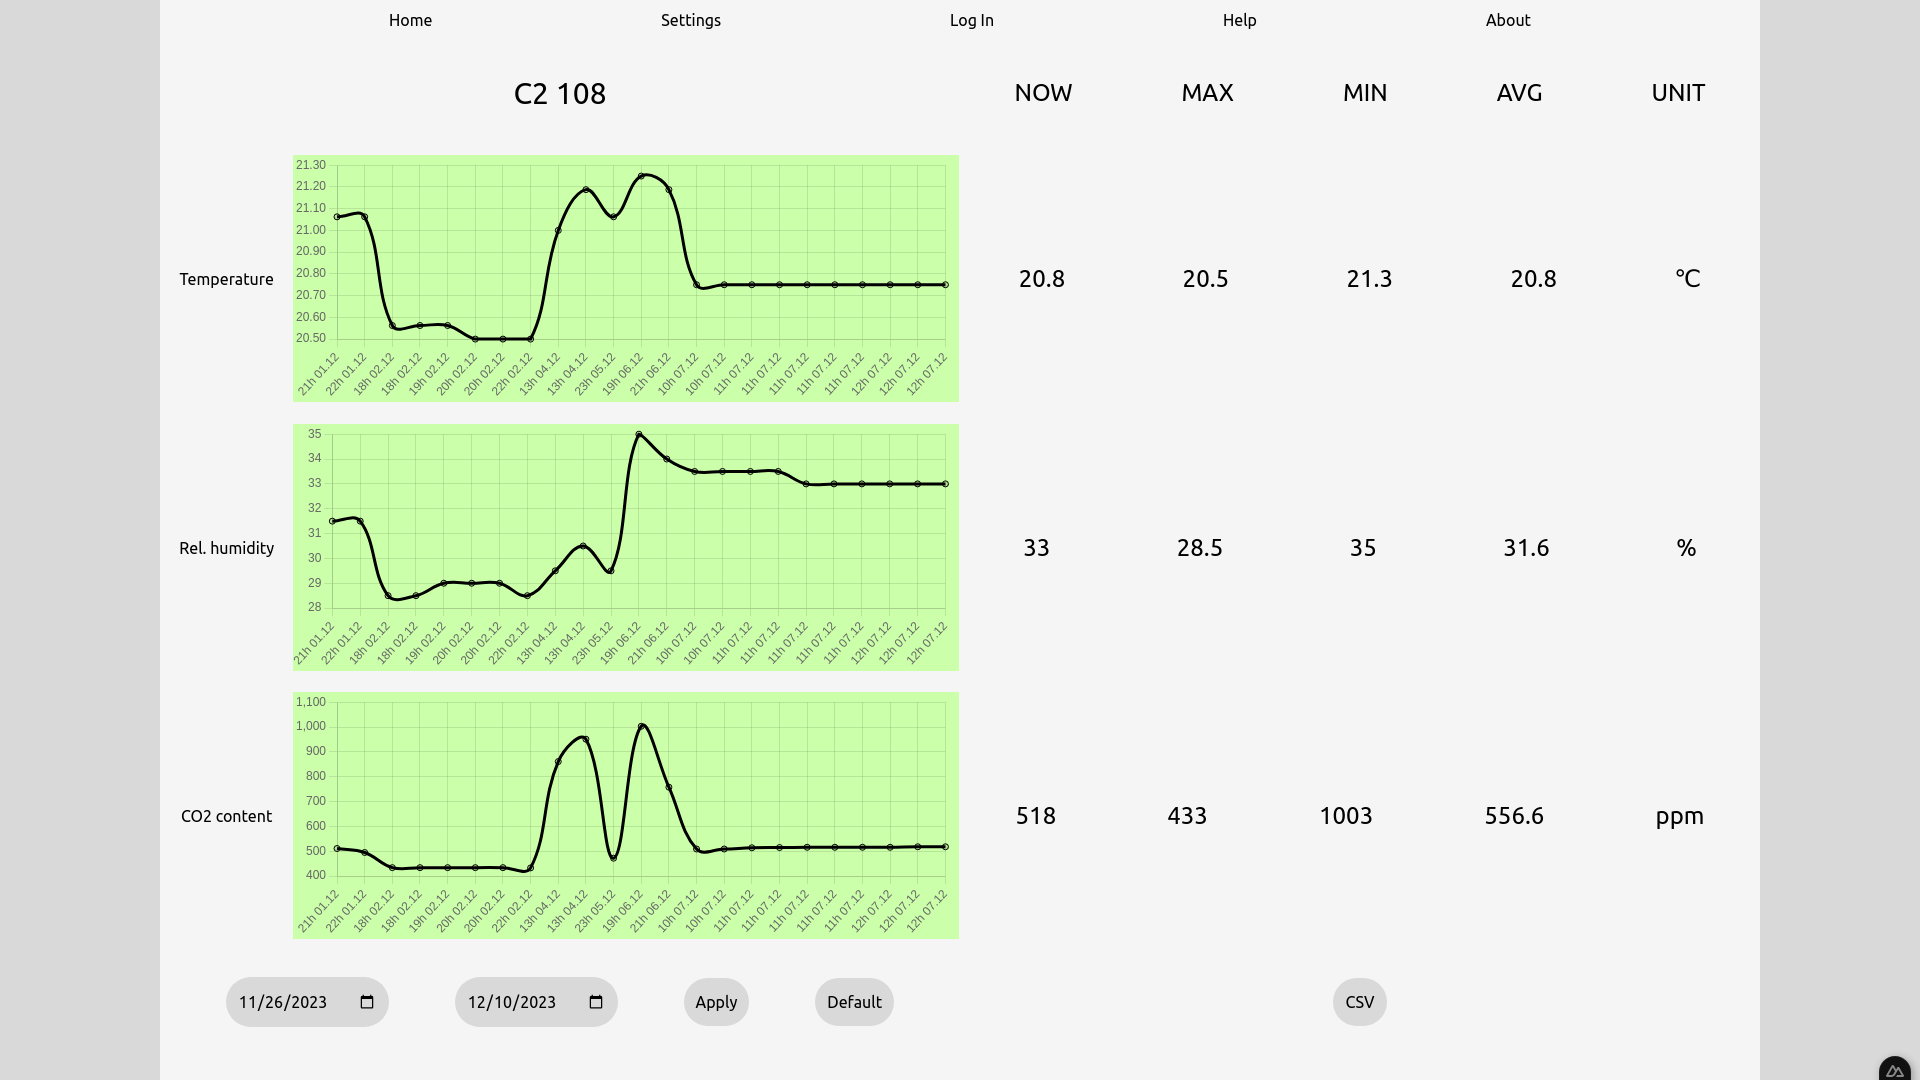
\includegraphics[width=\textwidth]{zdj/app/details.png}
    \caption{Zrzut ekranu przedstawiający widok szczegółów}
\end{figure}

Wybór zakresu odbywa się poprzez wybranie dwóch dat - początkowej i końcowej - w lewej dolnej części widoku. Daty można wpisać ręcznie lub posłużyć się
selektorem dat pojawiającym się po naciśnięciu w element. Aby wyświetlić dane z wybranego przedziału należy kliknąć w przycisk "Apply", po czym z serwera pobierane
są odpowiednie dane i ładowane do widoku. W tym trybie nowe dane nie są pobierane z serwera. 
Aby powrócić do domyślnej formy prezentowania odczytów (ładowanie danych na bieżąco) należy nacisnąć przycisk "Default". Bieżące oraz zaległe dane z odczytów
zaczną znowu być ładowane do widoku.

\begin{figure}[H]
    \centering
    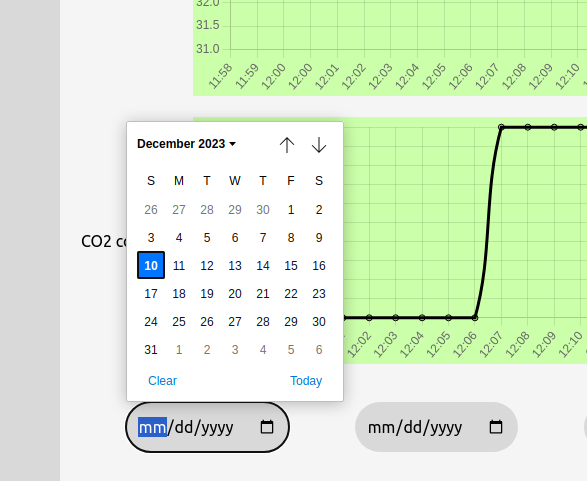
\includegraphics[width=0.5\textwidth]{zdj/app/date-pick.png}
    \caption{Wybieranie daty}
\end{figure}

\begin{figure}[H]
    \centering
    \begin{subfigure}{0.7\textwidth}
        \centering
        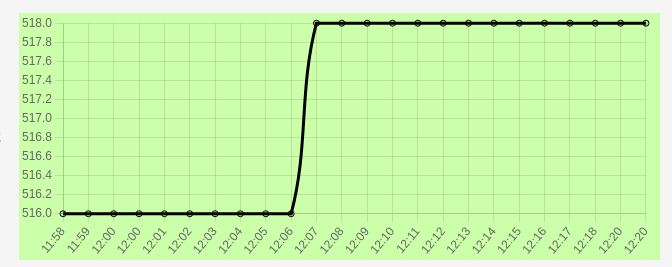
\includegraphics[width=\linewidth]{zdj/app/time-unit1.png}
        \caption{Jednostki w trybie domyślnym (24 najnowszych rekordów)}
    \end{subfigure}
    \begin{subfigure}{0.7\textwidth}
        \centering
        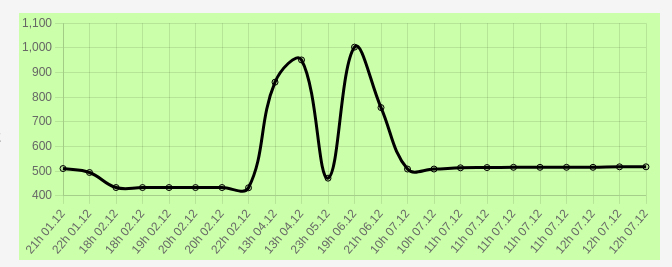
\includegraphics[width=\linewidth]{zdj/app/time-unit2.png}
        \caption{Jednostki po wybraniu okresu z ostatniego tygodnia}
    \end{subfigure}
       
    \caption{Schematy porównujące obie topologie sieci}
\end{figure}
W celu pobrania danych z wyznaczonego zakresu w postaci pliku CSV należy nacisnąć na przycisk "CSV". Otworzy to okienko pozwalające użytkownikowi wybranie folderu
zapisu pliku oraz zmianę jego nazwy. 

\begin{figure}[H]
    \centering
    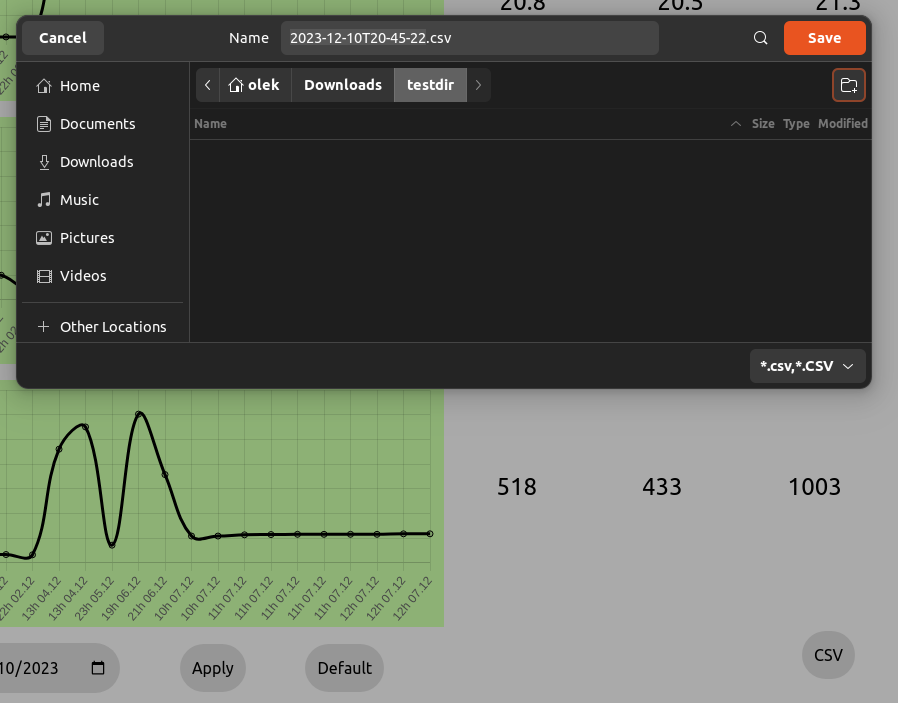
\includegraphics[width=0.6\textwidth]{zdj/app/download-csv.png}
    \caption{Pobieranie danych na komputer użytkownika}
\end{figure}

\subsection{Widok prezentacyjny}
Aplikacja posiada również widok pozwalający na czytelne i estetyczne zaprezentowanie danych bliżej nie określonej grupie odbiorców, na przykład poprzez wyświetlenie
na telewizorze na korytarzu.
Widok ten przedstawia odczyt z 4 czujników jednocześnie. Typ odczytu zmienia się cyklicznie co 20 sekund przedstawiając kolejno odczyty temperatury, wilgotności
i dwutlenku węgla

\begin{figure}[H]
    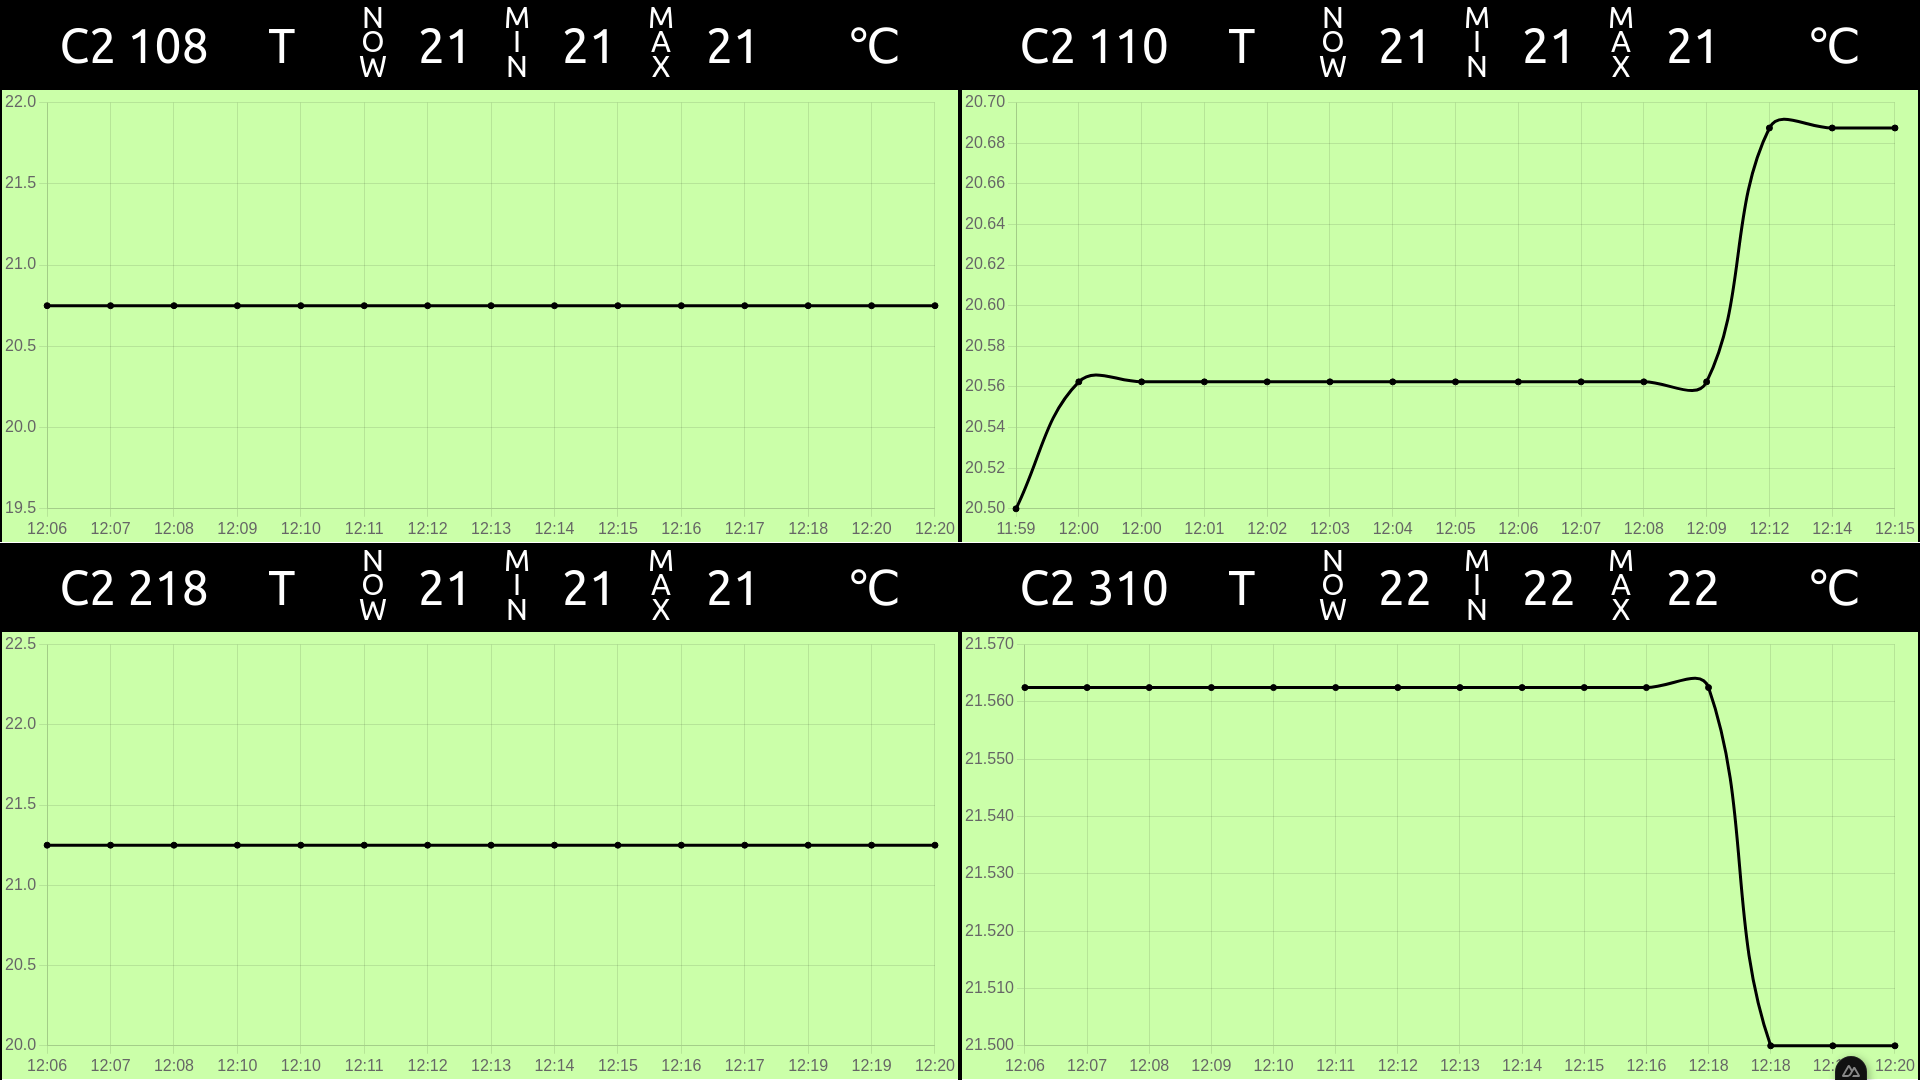
\includegraphics[width=\textwidth]{zdj/app/presentation-view.png}
    \caption{Zrzut ekranu widoku prezentacyjnego. Równe wartości niektórych punktów pomiarowych spowodowane
    są wysoką częstotliwością pollingu}
\end{figure}

W górnej części każdego z czterech elementów można odczytać podstawowe informacje, takie jak sala w której czujnik aktualnie się znajduje, typ odczytu, podstawowe
statystyki oraz jednostkę. Na każdym wykresie umieszczono horyzontalne linie odpowiadające poziomom komfortu odczytu. Tak jak w przypadku pozostałych widoków
dane wczytywane są na bieżąco - dostarczenie przez serwer nowej paczki odczytów spowoduje odświeżenie wykresów.